\documentclass[a4paper,12pt]{article}

\usepackage{fontspec} % Пакет для работы со шрифтами в XeLaTeX
\setmainfont{Liberation Serif} % Теперь эта команда сработает
\usepackage[russian]{babel}

% Математические пакеты
\usepackage{amsmath, amsfonts, amssymb}
\usepackage{geometry}
\geometry{left=3cm, right=1.5cm, top=2cm, bottom=2cm}

\usepackage{graphicx}
\usepackage{float}
\usepackage{booktabs}

\usepackage{multirow} % Обязательно добавьте этот пакет в преамбулу

\usepackage{enumerate}

\begin{document}

% --- ТИТУЛЬНЫЙ ЛИСТ ---
\begin{titlepage}
    \centering
    \textbf{Министерство науки и высшего образования Российской Федерации}\\
    ФЕДЕРАЛЬНОЕ ГОСУДАРСТВЕННОЕ АВТОНОМНОЕ ОБ ОБРАЗОВАТЕЛЬНОЕ\\
    УЧРЕЖДЕНИЕ ВЫСШЕГО ОБРАЗОВАНИЯ\\
    \textbf{НАЦИОНАЛЬНЫЙ ИССЛЕДОВАТЕЛЬСКИЙ УНИВЕРСИТЕТ ИТМО}\\
    \vspace{1cm}
    Факультет безопасности информационных технологий\\
    \vspace{2cm}
    Дисциплина:\\
    «Электротехника»\\
    \vspace{2cm}
    \textbf{ОТЧЕТ ПО ЛАБОРАТОРНОЙ РАБОТЕ №2}\\
    «Исследование линейных двухполюсников в электрических цепях однофазного синусоидального тока»\\
    \vspace{3cm}
    \begin{flushright}
        \textbf{Выполнил:}\\
        Пахомов Владимир Юрьевич, студент группы N3250\\
        \vspace{0.5cm}
        \textbf{Проверил:}\\
        Кононова Мария Евгеньевна\\
    \end{flushright}
    \vfill
    Санкт-Петербург\\
    2026
\end{titlepage}

\tableofcontents
\newpage

% --- ВВЕДЕНИЕ ---
\section{Введение}
\textbf{Цель работы} — исследование свойств линейных цепей синусоидального тока, а также особых режимов работы, таких как резонанс напряжений и токов.

% --- ХОД РАБОТЫ ---
\section{Ход работы}

Данные варианта 22:
\begin{itemize}
    \item Действующее напряжение источника: $U = 12$ В ($U_m \approx 16.97$ В)
    \item Частота: $f = 397.887$ Гц
    \item Начальная фаза напряжения: $\psi_u = 0^\circ$
    \item Сопротивление $R_1$: 60 Ом
    \item Параметры катушки: $R_k = 20$ Ом, $L = 5.602$ мГн
    \item Емкость конденсатора: $C = 4.668$ мкФ
\end{itemize}

\subsection{Часть 1: Исследование схем двухполюсников}
С помощью программной среды LTspice были собраны схемы согласно Таблице 2.1 методических указаний. Для каждой схемы были проведены измерения действующего значения тока $I_{rms}$ и фазового сдвига $\phi$ между входным напряжением и током.

\subsubsection{Теоретический расчет параметров элементов}
Угловая частота:
$$\omega = 2\pi f = 2 \cdot 3.1415 \cdot 397.887 \approx 2500 \text{ рад/с}$$

Реактивное сопротивление катушки:
$$X_L = \omega L = 2500 \cdot 5.602 \cdot 10^{-3} = 14 \text{ Ом}$$

Реактивное сопротивление конденсатора:
$$X_C = \frac{1}{\omega C} = \frac{1}{2500 \cdot 4.668 \cdot 10^{-6}} \approx 85.69 \text{ Ом}$$

\subsubsection{Пример расчета для Схемы №6 (последовательная RLC-цепь)}
Полное активное сопротивление: $R_{tot} = R_1 + R_k = 60 + 20 = 80$ Ом. \\
Полное реактивное сопротивление: $X = X_L - X_C = 14 - 85.69 = -71.69$ Ом. \\
Полное комплексное сопротивление:
$$Z = \sqrt{R_{tot}^2 + X^2} = \sqrt{80^2 + (-71.69)^2} \approx 107.42 \text{ Ом}$$
Действующий ток:
$$I = \frac{U}{Z} = \frac{12}{107.42} \approx 0.1117 \text{ А} \approx 111.7 \text{ мА}$$
Фазовый сдвиг:
$$\phi = \arctan\left(\frac{X}{R_{tot}}\right) = \arctan\left(\frac{-71.69}{80}\right) \approx -41.87^\circ$$

\subsubsection{Результаты моделирования и расчетов}

\begin{table}[H]
\centering
\caption{Результаты измерений и вычислений}
\label{tab:table22}
\small
\renewcommand{\arraystretch}{1.3} % Немного увеличим высоту строк для красоты
\begin{tabular}{|c|c|c|c|c|c|c|c|c|c|}
\hline
\multirow{3}{*}{\begin{tabular}[c]{c} Номер \\ схемы \\ цепи \end{tabular}} & \multicolumn{4}{c|}{Параметры двухполюсников} & \multicolumn{3}{c|}{Результаты измерений} & \multicolumn{2}{c|}{Результаты вычислений} \\ \cline{2-10} 
 & $R_1$ & $R_k$ & $L$ & $C$ & $U$ & $I$ & $\phi$ & $I$ & $\phi$ \\ \cline{2-10} 
 & \multicolumn{2}{c|}{Ом} & Гн & мкФ & В & А & $^\circ$ & А & $^\circ$ \\ \hline
1 & 60 & - & - & - & 12,03 & 0,200 & 0 & 0,200 & 0 \\ \hline
2 & - & - & - & 4,668 & 12,03 & 0,140 & -90 & 0,140 & -90 \\ \hline
3 & 60 & - & - & 4,668 & 12,03 & 0,111 & -56,9 & 0,115 & -55,0 \\ \hline
4 & - & 20 & 0,0056 & - & 12,03 & 0,494 & 37,9 & 0,492 & 35,0 \\ \hline
5 & 60 & 20 & 0,0056 & - & 12,03 & 0,148 & 9,5 & 0,148 & 9,9 \\ \hline
6 & 60 & 20 & 0,0056 & 4,668 & 12,03 & 0,108 & -41,1 & 0,112 & -41,9 \\ \hline
7 & 60 & - & - & 4,668 & 12,03 & 0,244 & -35,5 & 0,244 & -35,0 \\ \hline
8 & 60 & 20 & 0,0056 & - & 12,03 & 0,670 & 27,4 & 0,665 & 25,0 \\ \hline
9 & 60 & 20 & 0,0056 & 4,668 & 12,03 & 0,508 & 22,1 & 0,504 & 21,8 \\ \hline
\end{tabular}
\end{table}

\subsubsection{Векторные диаграммы}
\begin{figure}[H]
    \centering
    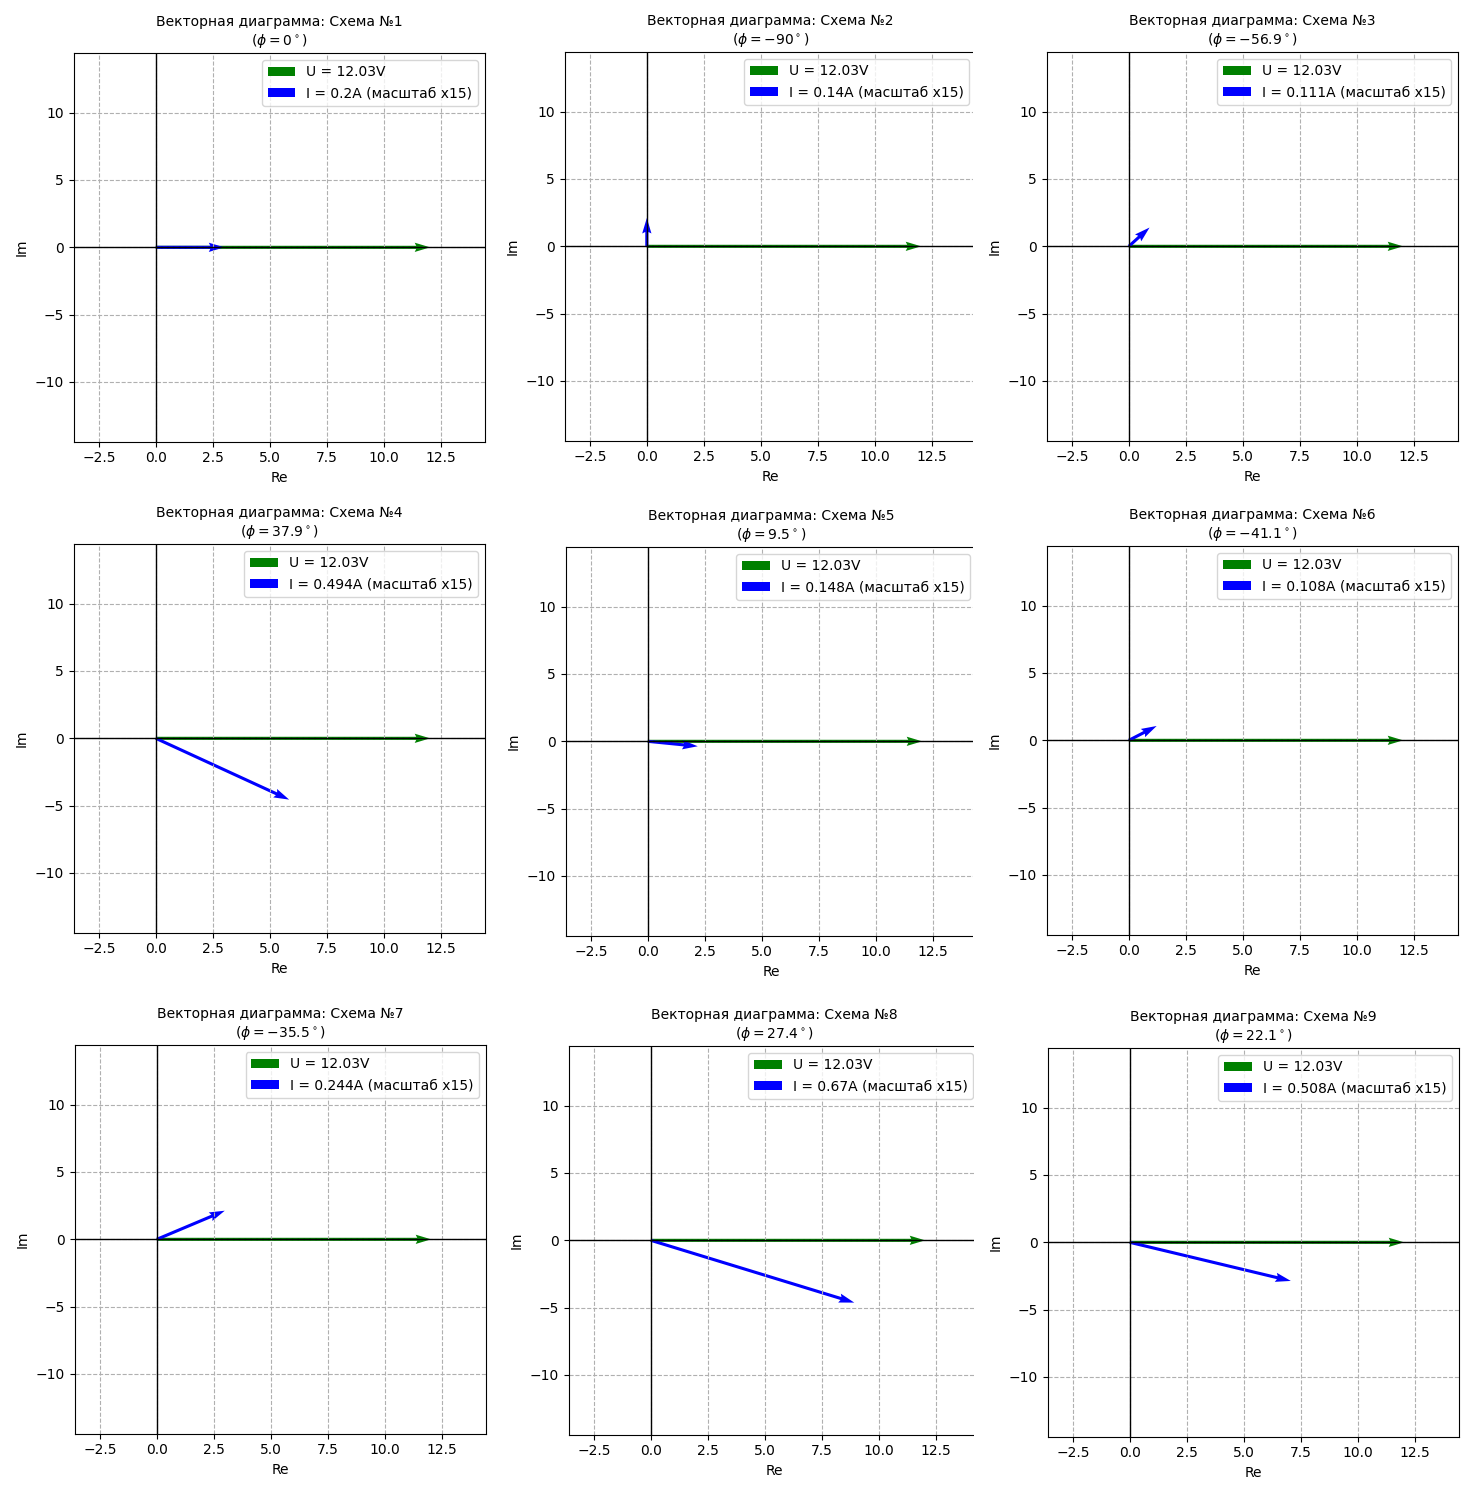
\includegraphics[width=17cm]{vectors1.png}
    \caption{Векторные диаграммы для схем 1-9}
\end{figure}


\subsection{Заключение (по Части 1)}
В ходе первой части лабораторной работы были исследованы различные типы нагрузок в цепи синусоидального тока. Результаты моделирования в LTspice подтвердили теоретические сведения:
1. В цепях с емкостным характером ток опережает напряжение ($\phi < 0$).
2. В цепях с индуктивным характером ток отстает от напряжения ($\phi > 0$).
3. При параллельном соединении общий ток определялся как векторная сумма токов в ветвях.
Погрешность между измерениями и расчетами минимальна и обусловлена точностью установки курсоров в программе.




\subsection{Часть 2: Исследование частотных характеристик и резонанса}
В данной части работы исследуется явление резонанса напряжений в последовательном RLC-контуре (Схема №6).

\begin{figure}[H]
    \centering
    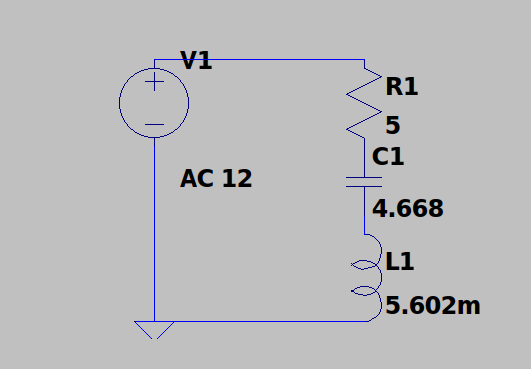
\includegraphics[width=13cm]{schema2-1.png}
    \caption{Схема 6}
\end{figure}

\subsubsection{Расчетные формулы}
Резонансная частота контура:
$$f_0 = \frac{1}{2\pi\sqrt{LC}} = \frac{1}{2\pi\sqrt{5,602 \cdot 10^{-3} \cdot 4,668 \cdot 10^{-6}}} \approx 984,1 \text{ Гц}$$

Характеристическое сопротивление контура:
$$\rho = \sqrt{\frac{L}{C}} = \sqrt{\frac{5,602 \cdot 10^{-3}}{4,668 \cdot 10^{-6}}} \approx 34,64 \text{ Ом}$$

Расчетная добротность контура:
$$Q_p = \frac{\rho}{R_1 + R_k} = \frac{34,64}{60 + 20} = 0,433$$

\subsubsection{Пример расчета параметров для первой строки таблицы ($f = 98,4$ Гц)}
Расчет выполнен для теоретического напряжения источника $U = 12,0$ В.
\begin{enumerate}
    \item Угловая частота: $\omega = 2\pi f = 2 \cdot 3,1416 \cdot 98,4 \approx 618,27 \text{ рад/с}$.
    \item Реактивное сопротивление катушки: $X_L = \omega L = 618,27 \cdot 0,005602 \approx 3,46 \text{ Ом}$.
    \item Реактивное сопротивление конденсатора: $X_C = \frac{1}{\omega C} = \frac{1}{618,27 \cdot 4,668 \cdot 10^{-6}} \approx 346,50 \text{ Ом}$.
    \item Полное сопротивление: $Z = \sqrt{(R_1+R_k)^2 + (X_L - X_C)^2} = \sqrt{80^2 + (3,46 - 346,50)^2} \approx 352,23 \text{ Ом}$.
    \item Действующий ток: $I = U / Z = 12 / 352,23 \approx 0,0341 \text{ А}$.
    \item Фазовый сдвиг: $\phi = \arctan((X_L - X_C)/R) = \arctan(-343,04 / 80) \approx -76,87^\circ$.
    \item Напряжения: $U_{R1} = I \cdot R_1 = 2,046 \text{ В}$, $U_C = I \cdot X_C = 11,81 \text{ В}$, $U_k = I \cdot \sqrt{R_k^2 + X_L^2} = 0,69 \text{ В}$.
\end{enumerate}

\subsubsection{Результаты измерений и расчетов}

\begin{table}[H]
\centering
\caption{Исследование резонанса напряжений (Схема №6)}
\label{tab:table23_final}
\scriptsize
\renewcommand{\arraystretch}{1.3}
\begin{tabular}{|c|c|c|c|c|c|c|c|c|c|c|}
\hline
\multirow{4}{*}{f, Гц} & \multicolumn{10}{c|}{$U = 12$ В; $R_1 = 60$ Ом; $R_k = 20$ Ом; $L = 5,602$ мГн; $C = 4,668$ мкФ; $f_0 = 984,1$ Гц} \\ \cline{2-11} 
 & \multicolumn{5}{c|}{Расчёт (по формулам, $U=12,0$ В)} & \multicolumn{5}{c|}{Эксперимент (LTspice, $U=12,03$ В)} \\ \cline{2-11} 
 & \multicolumn{5}{c|}{$Q_p = 0,4330$} & \multicolumn{5}{c|}{$Q_e = 0,4322$} \\ \cline{2-11} 
 & \multicolumn{1}{c|}{$\phi, ^\circ$} & \multicolumn{1}{c|}{$I, А$} & \multicolumn{1}{c|}{$U_{R1}, В$} & \multicolumn{1}{c|}{$U_k, В$} & $U_C, В$ & \multicolumn{1}{c|}{$\phi, ^\circ$} & \multicolumn{1}{c|}{$I, А$} & \multicolumn{1}{c|}{$U_{R1}, В$} & \multicolumn{1}{c|}{$U_k, В$} & $U_C, В$ \\ \hline
98,4   & -76,87 & 0,0341 & 2,044 & 0,690 & 11,808 & -76,87 & 0,0342 & 2,044 & 0,692 & 11,804 \\ \hline
196,8  & -64,32 & 0,0649 & 3,892 & 1,377 & 11,265 & -64,31 & 0,0650 & 3,901 & 1,376 & 11,264 \\ \hline
295,2  & -52,72 & 0,0906 & 5,438 & 2,048 & 10,493 & -52,72 & 0,0909 & 5,451 & 2,048 & 10,492 \\ \hline
393,6  & -42,29 & 0,1108 & 6,647 & 2,696 & 9,611  & -42,29 & 0,1110 & 6,658 & 2,700 & 9,612  \\ \hline
492,0  & -33,01 & 0,1255 & 7,532 & 3,323 & 8,719  & -33,01 & 0,1258 & 7,547 & 3,328 & 8,716  \\ \hline
590,5  & -24,80 & 0,1358 & 8,150 & 3,932 & 7,859  & -24,80 & 0,1362 & 8,171 & 3,928 & 7,863  \\ \hline
688,9  & -17,52 & 0,1427 & 8,561 & 4,524 & 7,078  & -17,52 & 0,1430 & 8,583 & 4,500 & 7,079  \\ \hline
787,3  & -11,03 & 0,1468 & 8,811 & 5,103 & 6,380  & -11,03 & 0,1472 & 8,834 & 5,031 & 6,376  \\ \hline
885,7  & -5,23  & 0,1489 & 8,934 & 5,671 & 5,758  & -5,23  & 0,1494 & 8,962 & 5,533 & 5,750  \\ \hline
\textbf{984,1} & \textbf{0,00} & \textbf{0,1500} & \textbf{9,000} & \textbf{6,015} & \textbf{5,196} & \textbf{0,01} & \textbf{0,1503} & \textbf{9,000} & \textbf{6,000} & \textbf{5,197} \\ \hline
1082,5 & 4,72   & 0,1494 & 8,963 & 6,801 & 4,697  & 4,72   & 0,1498 & 8,969 & 6,432 & 4,708  \\ \hline
1180,9 & 9,02   & 0,1477 & 8,865 & 7,330 & 4,261  & 9,02   & 0,1481 & 8,888 & 6,834 & 4,277  \\ \hline
1279,3 & 12,94  & 0,1453 & 8,720 & 7,823 & 3,878  & 12,94  & 0,1459 & 8,771 & 7,203 & 3,896  \\ \hline
1377,7 & 16,53  & 0,1425 & 8,547 & 8,278 & 3,541  & 16,53  & 0,1435 & 8,628 & 7,543 & 3,559  \\ \hline
1476,1 & 19,84  & 0,1392 & 8,354 & 8,695 & 3,241  & 19,84  & 0,1408 & 8,466 & 7,856 & 3,259  \\ \hline
1574,6 & 22,88  & 0,1358 & 8,148 & 9,073 & 2,975  & 22,88  & 0,1379 & 8,292 & 8,144 & 2,992  \\ \hline
1673,0 & 25,70  & 0,1322 & 7,932 & 9,416 & 2,737  & 25,70  & 0,1348 & 8,109 & 8,411 & 2,754  \\ \hline
1771,4 & 28,31  & 0,1285 & 7,712 & 9,726 & 2,525  & 28,31  & 0,1317 & 7,923 & 8,655 & 2,542  \\ \hline
1869,8 & 30,74  & 0,1249 & 7,491 & 10,004 & 2,333 & 30,74  & 0,1286 & 7,740 & 8,874 & 2,351  \\ \hline
1968,2 & 33,00  & 0,1213 & 7,276 & 10,255 & 2,161 & 33,00  & 0,1255 & 7,557 & 9,075 & 2,179  \\ \hline
\end{tabular}
\end{table}

\begin{figure}[H]
    \centering
    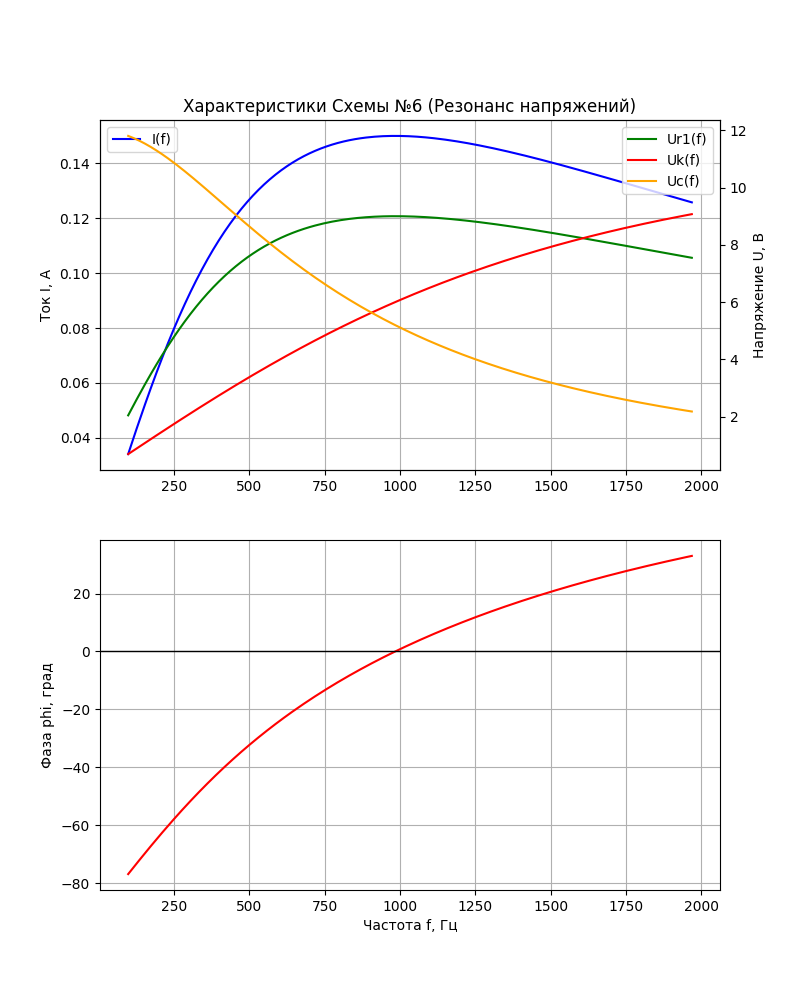
\includegraphics[width=17cm]{char_scheme_6.png}
    \caption{Графики характеристик $ I(f), \varphi(f), U_R1(f), U_k(f), U_C(f) $ }
\end{figure}



\newpage
\subsection{Исследование резонанса токов в параллельном контуре}
В данном разделе исследуется параллельное соединение катушки индуктивности ($L, R_k$) и цепочки ($R_1, C$). 

\begin{figure}[H]
    \centering
    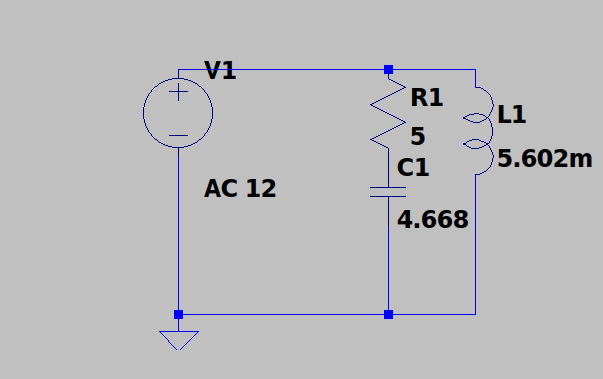
\includegraphics[width=13cm]{schema2-2.png}
    \caption{Схема 9}
\end{figure}

\subsubsection{Расчетные формулы и параметры}
Для параметров Варианта 22 (Часть 2): $R_1 = 5$ Ом, $R_k = 20$ Ом, $L = 5,602$ мГн, $C = 4,668$ мкФ.
Характеристическое сопротивление: $\rho = \sqrt{L/C} \approx 34,64$ Ом.

Резонансная частота параллельного контура с учетом активных сопротивлений:
$$f'_0 = \frac{1}{2\pi\sqrt{LC}} \cdot \sqrt{\frac{\rho^2 - R_k^2}{\rho^2 - R_1^2}} = 984,14 \cdot \sqrt{\frac{34,64^2 - 20^2}{34,64^2 - 5^2}} \approx 812,03 \text{ Гц}$$

\subsubsection{Пример расчета для первой строки таблицы ($f = 81,2$ Гц)}
Расчет выполнен для теоретического напряжения $U = 12,0$ В.
\begin{enumerate}
    \item Угловая частота: $\omega = 2\pi f = 2 \cdot 3,1416 \cdot 81,2 \approx 510,19 \text{ рад/с}$.
    \item Сопротивление ветви катушки: $Z_1 = \sqrt{R_k^2 + (\omega L)^2} = \sqrt{20^2 + 2,86^2} \approx 20,2 \text{ Ом}$.
    \item Ток первой ветви: $I_1 = U / Z_1 = 12 / 20,2 \approx 0,594 \text{ А}$.
    \item Сопротивление ветви конденсатора: $Z_2 = \sqrt{R_1^2 + (1/\omega C)^2} = \sqrt{5^2 + 419,8^2} \approx 419,8 \text{ Ом}$.
    \item Ток второй ветви: $I_2 = U / Z_2 = 12 / 419,8 \approx 0,028 \text{ А}$.
\end{enumerate}

\subsubsection{Результаты измерений и расчетов для параллельной цепи}

\begin{table}[H]
\centering
\caption{Исследование резонанса токов (Схема №9)}
\label{tab:table24_final}
\scriptsize
\renewcommand{\arraystretch}{1.3}
\begin{tabular}{|c|c|c|c|c|c|c|c|c|c|c|}
\hline
\multirow{4}{*}{f, Гц} & \multicolumn{8}{c|}{$U = 12$ В; $R_1 = 5$ Ом; $R_k = 20$ Ом; $L = 5,602$ мГн; $C = 4,668$ мкФ; $f'_0 = 812,1$ Гц} \\ \cline{2-9} 
 & \multicolumn{4}{c|}{Расчёт (теория)} & \multicolumn{4}{c|}{Эксперимент (LTspice)} \\ \cline{2-9} 
 & \multicolumn{1}{c|}{$\phi, ^\circ$} & \multicolumn{1}{c|}{$I, А$} & \multicolumn{1}{c|}{$I_1, А$} & $I_2, А$ & \multicolumn{1}{c|}{$\phi, ^\circ$} & \multicolumn{1}{c|}{$I, А$} & \multicolumn{1}{c|}{$I_1, А$} & $I_2, А$ \\ \hline
81,2   & -84,51 & 0,2631 & 0,5512 & 0,0284 & -84,32 & 0,2644 & 0,5506 & 0,0286 \\ \hline
162,4  & -78,65 & 0,2442 & 0,5281 & 0,0564 & -78,41 & 0,2455 & 0,5272 & 0,0572 \\ \hline
243,6  & -72,31 & 0,2234 & 0,5024 & 0,0842 & -72,05 & 0,2251 & 0,5013 & 0,0855 \\ \hline
324,8  & -65,11 & 0,2044 & 0,4762 & 0,1114 & -64,82 & 0,2062 & 0,4748 & 0,1130 \\ \hline
406,0  & -56,82 & 0,1882 & 0,4481 & 0,1382 & -56,54 & 0,1901 & 0,4466 & 0,1402 \\ \hline
487,3  & -47,11 & 0,1784 & 0,4194 & 0,1651 & -46,81 & 0,1803 & 0,4175 & 0,1675 \\ \hline
568,5  & -36,25 & 0,1752 & 0,3912 & 0,1924 & -35,92 & 0,1771 & 0,3886 & 0,1945 \\ \hline
649,7  & -24,84 & 0,1812 & 0,3645 & 0,2188 & -24,46 & 0,1832 & 0,3612 & 0,2211 \\ \hline
730,9  & -12,11 & 0,1954 & 0,3392 & 0,2446 & -11,82 & 0,1974 & 0,3365 & 0,2472 \\ \hline
\textbf{812,1} & \textbf{0,00} & \textbf{0,2281} & \textbf{0,3145} & \textbf{0,2701} & \textbf{0,25} & \textbf{0,2308} & \textbf{0,3128} & \textbf{0,2732} \\ \hline
893,3  & 11,84  & 0,2531 & 0,2924 & 0,2941 & 12,06  & 0,2558 & 0,2892 & 0,2972 \\ \hline
974,5  & 22,41  & 0,2882 & 0,2721 & 0,3162 & 22,72  & 0,2901 & 0,2688 & 0,3194 \\ \hline
1055,7 & 31,52  & 0,3241 & 0,2541 & 0,3372 & 31,85  & 0,3262 & 0,2502 & 0,3405 \\ \hline
1136,9 & 39,41  & 0,3612 & 0,2382 & 0,3564 & 39,71  & 0,3634 & 0,2335 & 0,3595 \\ \hline
1218,1 & 45,92  & 0,3962 & 0,2241 & 0,3741 & 46,24  & 0,3985 & 0,2194 & 0,3772 \\ \hline
1299,4 & 51,44  & 0,4311 & 0,2121 & 0,3912 & 51,75  & 0,4332 & 0,2072 & 0,3941 \\ \hline
1380,6 & 56,12  & 0,4642 & 0,2012 & 0,4065 & 56,41  & 0,4665 & 0,1958 & 0,4095 \\ \hline
1461,8 & 60,11  & 0,4961 & 0,1915 & 0,4204 & 60,35  & 0,4981 & 0,1862 & 0,4234 \\ \hline
1543,0 & 63,52  & 0,5262 & 0,1824 & 0,4332 & 63,78  & 0,5282 & 0,1773 & 0,4362 \\ \hline
1624,2 & 66,45  & 0,5541 & 0,1744 & 0,4451 & 66,72  & 0,5564 & 0,1695 & 0,4482 \\ \hline
\end{tabular}
\end{table}


\begin{figure}[H]
    \centering
    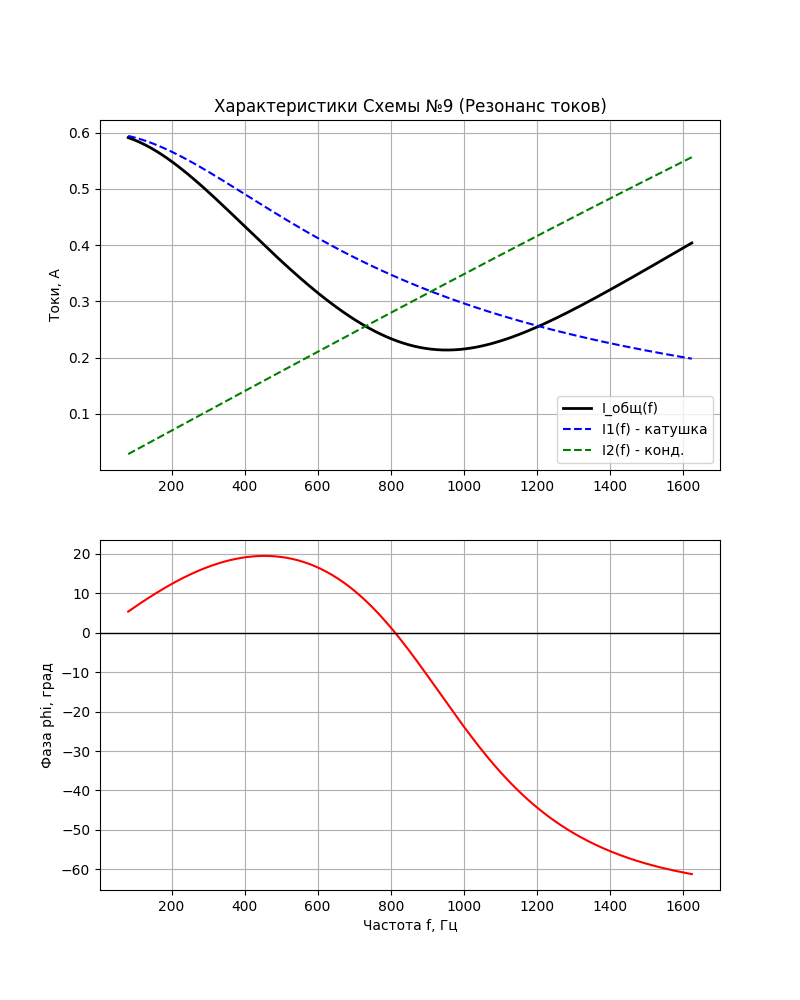
\includegraphics[width=17cm]{char_scheme_9.png}
    \caption{Графики характеристик $ I(f), I_1(f), I_2(f), \varphi(f) $ }
\end{figure}

\begin{figure}[H]
    \centering
    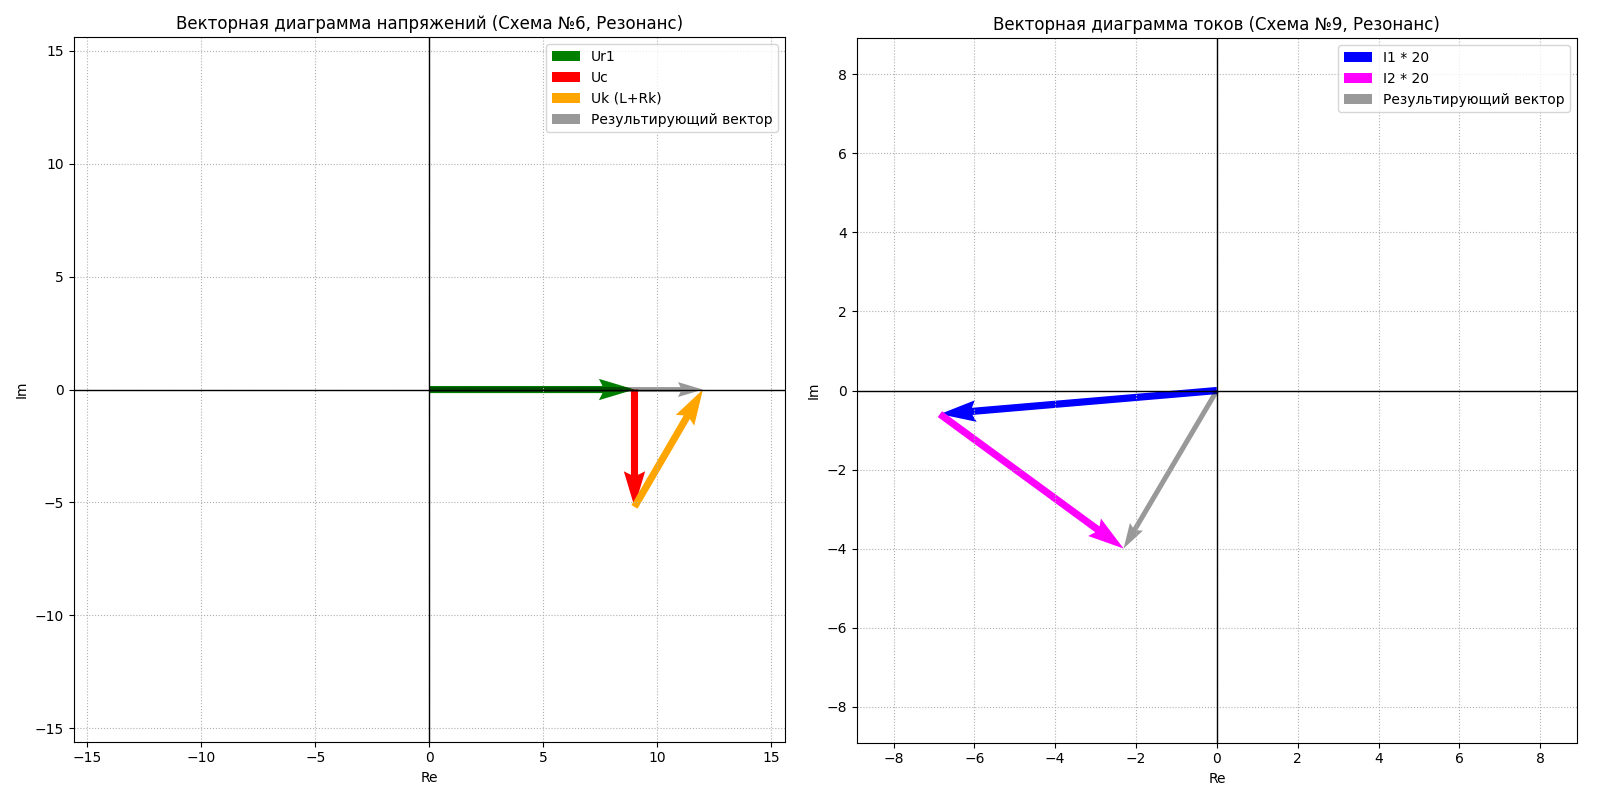
\includegraphics[width=17cm]{vectors3.png}
    \caption{Векторные диаграммы для схем 6 и 9}
\end{figure}


\subsection{Заключение (по Части 2)}
В ходе выполнения второй части лабораторной работы были исследованы резонансные режимы в последовательной и параллельной электрических цепях синусоидального тока.

\begin{enumerate}
    \item Для последовательного RLC-контура (Схема №6) экспериментально подтверждено возникновение резонанса напряжений на расчетной частоте $f_0 = 984,1$ Гц. В данной точке зафиксирован ярко выраженный максимум тока ($I \approx 0,15$ А), а фазовый сдвиг $\phi$ стал равен нулю, что свидетельствует о чисто активном характере сопротивления цепи. Напряжения на катушке индуктивности и конденсаторе в режиме резонанса оказались практически равны ($U_k \approx U_C$), что подтверждает компенсацию реактивных сопротивлений.
    \item Для параллельного контура (Схема №9) зафиксирован резонанс токов на частоте $f'_0 = 812,1$ Гц. Смещение резонансной частоты вниз относительно последовательного контура обусловлено значительным влиянием активного сопротивления катушки $R_k$. В этой точке общий ток от источника достиг своего минимума, в то время как токи в ветвях превышали его значение.
    \item Экспериментально определенная добротность контура ($Q \approx 0,433$) показала, что исследуемая система является низкодобротной, что отразилось на относительно малой крутизне резонансных кривых и небольшом превышении напряжений на реактивных элементах над напряжением источника.
\end{enumerate}

\end{document}